% format: pdflatex
% TikZ and tikz-cd: most of the expansion a document can ask for, floating point in macros, and PDF literals.  A plain square with new letters.
\pdfinfoomitdate=1
\pdftrailerid{}
\documentclass{article}
\usepackage{tikz-cd}
\begin{document}
\begin{tikzcd}
P \arrow[r, "u"] \arrow[d, "v"'] & Q \arrow[d, "w"] \\
R \arrow[r, "z"'] & S
\end{tikzcd}

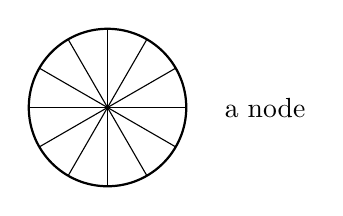
\begin{tikzpicture}
\draw[thick] (0,0) circle (1cm);
\foreach \a in {0,30,...,330} \draw (0,0) -- (\a:1cm);
\node at (2,0) {a node};
\end{tikzpicture}
\end{document}
